\documentclass[10pt]{article}
\usepackage[margin=1.35in]{geometry}
\usepackage{times}
\usepackage{mathptmx}
\usepackage{amsmath,amssymb}
\usepackage{booktabs}
\usepackage{graphicx}
\usepackage{tikz}
\usepackage{pgfplots}
\pgfplotsset{compat=1.16}
\usetikzlibrary{arrows.meta,positioning,fit,backgrounds,calc}
\usepackage[numbers,sort&compress]{natbib}
\usepackage[hidelinks]{hyperref}
\usepackage{caption}
\captionsetup{font=small,labelfont=bf}
\usepackage{authblk}

\renewcommand{\baselinestretch}{1.0}
\setlength{\parskip}{2pt}

\title{\bf Structure-Conditioned Pretraining for Genomic Sequence Models:\\
A Timescale Ceiling and a Diagnosed Null}

\author[ ]{Author One}
\author[ ]{Author Two}
\affil[ ]{\small Affiliation\\\texttt{\{a.one, a.two\}@institution.edu}}
\date{}

\begin{document}
\maketitle

\begin{abstract}
\noindent
State-space sequence models are increasingly used as genomic foundation models
because their linear cost admits contexts far beyond attention. We report two
results about conditioning such a model on measured three-dimensional chromatin
structure during pretraining, rather than attaching structure to frozen
embeddings after the fact.

First, we identify a \emph{timescale ceiling} that is present before training
begins. In a selective state-space model the retention time obeys
$\tau = 1/(\Delta|A| + p)$, so the initialisation constants of $\Delta$ and of
any additive gate impose a hard upper bound on memory. With Mamba's reference
$\Delta_{\min} = 10^{-3}$ this bound is $10^{3}$ tokens, which at
single-nucleotide tokenisation is shorter than a typical gene; we measure
$999.5$. The ceiling is invisible to the standard diagnostic, which omits $p$.
Correcting three constants at \emph{zero} parameter cost moves median trained
$\tau$ from $14.2$ to $434.7$ and takes the fraction of layer-directions
reaching topological-domain scale from $0/32$ to $32/32$.

Second, with that ceiling removed, we find that conditioning $\Delta$ on
Hi-C-derived structure gives \emph{no} improvement in masked-language-modelling
loss at matched parameters and matched compute ($+0.0020$ bits, $0.80\sigma$,
exact permutation $p = 0.600$), and we diagnose why. The structural signal is
overwhelmingly \emph{between} windows rather than within them: only $11.0\%$ of
its variance lies inside a $65{,}536$\,bp window. We show this is a property of
Hi-C spatial autocorrelation and not of binning or window choice, by measuring
it three ways --- across window widths from $8$\,kb to $524$\,kb, across bin
resolutions from $5$\,kb to $1$\,kb, and through the structural encoder. A
per-position conditioning mechanism therefore addresses a minority of the
available signal by construction, at every resolution and context length
reachable on commodity hardware.
\end{abstract}

\section{Introduction}

The genome is read as a one-dimensional string but functions as a folded
three-dimensional object. Regulatory contacts routinely join loci hundreds of
kilobases apart in sequence that are adjacent in space, and this folding is
measurable: chromosome conformation capture (Hi-C) yields contact maps from
which topologically associating domains (TADs) and A/B compartments can be
derived \citep{liebermanaiden2009, rao2014}.

Sequence models for genomics have grown contexts aggressively, first with
efficient attention and more recently with state-space models (SSMs) whose cost
is linear in length \citep{gu2023mamba, nguyen2023hyenadna, schiff2024caduceus}.
A natural question follows: if a model must learn long-range dependence, and
that dependence is partly explained by measured folding, does supplying the
folding help?

Existing work answers this by \emph{post-hoc attachment}. Structure is applied
to representations that are already frozen, typically through graph attention
over a contact graph. This tests whether structure is useful for a downstream
readout, but it cannot test whether structure changes what the encoder learns.

We ask the other question. We inject structure \emph{during} pretraining, at the
one place in a selective SSM where long-range behaviour is actually decided: the
timescale $\Delta$, which sets how long the recurrent state retains information.
The hypothesis is direct --- a model told where domain boundaries are should
learn to reset at them and retain within them.

Answering it required first fixing something we did not expect to find. Our
contributions are:

\begin{itemize}
\itemsep2pt
\item \textbf{A timescale ceiling in SSM initialisation} (\S\ref{sec:ceiling}).
The reference $\Delta$ initialisation caps retention at $1/\Delta_{\min}$ tokens
before the first gradient step. The fix costs no parameters. We further show the
ceiling recurs through a second constant --- an additive gate term $p$ omitted
from the usual $\tau$ estimator --- which silently reimposes a $55$-token bound
on the conditioned model while leaving the unconditioned baseline untouched.
\item \textbf{A mechanism for structure-conditioned pretraining}
(\S\ref{sec:method}), costing $+0.43\%$ parameters and numerically identical to
its baseline at initialisation, so that anything observed is learned.
\item \textbf{A matched-parameter, matched-compute null, with controls}
(\S\ref{sec:results}). Loss is unchanged; input-substitution controls show the
structural channel reaches the output but carries $\sim\!0.05\%$ of the
divergence that masking does.
\item \textbf{A measured explanation} (\S\ref{sec:why}). The conditioning signal
is nearly constant inside the window it modulates, and we show this is intrinsic
to Hi-C rather than an artefact of binning or context length.
\end{itemize}

We report the null as a result. The design was pre-registered, the effect-size
floor was fixed before any number existed, and no threshold was moved
afterwards.

\section{Related work}

\paragraph{Long-context genomic sequence models.}
Attention-based genomic models are limited by quadratic cost, which at
single-nucleotide tokenisation binds quickly. Implicit-convolution and
state-space architectures relaxed this: HyenaDNA \citep{nguyen2023hyenadna}
reaches $10^{6}$-token contexts at single-nucleotide resolution, and Caduceus
\citep{schiff2024caduceus} adds reverse-complement equivariance to a
bidirectional Mamba backbone \citep{gu2023mamba}. Our backbone is deliberately
of this family and parameter-matched to the smallest published Caduceus
configuration, so that the mechanism rather than the scale is what differs.
The timescale ceiling of \S\ref{sec:ceiling} is a property of the shared
initialisation and therefore applies to this family generally, not only to the
model studied here.

\paragraph{Structure-aware genomic models.}
A second line predicts folding \emph{from} sequence: Akita and Orca learn
contact maps directly, establishing that sequence carries substantial
information about three-dimensional organisation. The converse direction ---
using measured folding to improve sequence representations --- has been
approached by attaching structure to representations that are already trained.
Graph-attention methods of this kind operate over a contact graph on top of
\emph{frozen} embeddings. This is an effective way to exploit structure at
readout time, but it leaves the encoder unchanged and therefore cannot answer
whether structure alters what is learned. Our design differs in exactly this
respect: conditioning is applied during pretraining and is removed at transfer
time, so any benefit must reside in the learned sequence weights.

\paragraph{Conditioning recurrent timescales.}
Gating a recurrent model's retention on side information has precedent in
general sequence modelling, where forget-gate biases control effective memory
length. What is specific here is the interpretation: in a selective SSM the
timescale is an explicit, measurable quantity in tokens, so an external signal
that predicts \emph{where dependencies end} --- which is what an insulation
profile is --- can be applied to it directly and its effect audited. That
auditability is what makes the negative result of \S\ref{sec:results}
diagnosable rather than merely disappointing.

\section{Background}

\paragraph{Selective state-space models.}
A selective SSM maintains a state $h_t$ updated as
$h_t = \bar{A}_t h_{t-1} + \bar{B}_t x_t$, where the discretisation
$\bar{A}_t = \exp(\Delta_t A)$ makes the effective retention time input
dependent. With $A$ diagonal and negative, the characteristic decay time of
direction $i$ is
\begin{equation}
\tau_{t,i} \;=\; \frac{1}{\Delta_t |A_i|}\,,
\label{eq:tau}
\end{equation}
so $\Delta$ is the quantity that decides how far back the model can see. In
Mamba, $\Delta_t = \mathrm{softplus}(W_\Delta x_t + b_\Delta)$, and $b_\Delta$ is
initialised so that $\Delta$ spans $[\Delta_{\min}, \Delta_{\max}]$.

\paragraph{Structural features.}
From a Hi-C contact matrix at $5$\,kb resolution we derive an eight-dimensional
per-bin vector $\varphi$: insulation at three scales ($100$, $250$, $500$\,kb),
a $2$\,Mb directionality index, log contact density, upstream mass fraction,
short-to-long range ratio, and the first principal component of the correlation
matrix (the A/B compartment eigenvector). Validated against independently
processed tracks, our insulation attains Pearson $r = 0.9969$ and our
compartment eigenvector $r = 0.9759$.

Under reverse complementation the features carry signs
$[1,1,1,-1,1,-1,1,1]$; directionality and upstream mass fraction are
antisymmetric. This flip must be applied to raw $\varphi$ before encoding, since
an encoder mixes the coordinates and destroys the correspondence.

\section{A timescale ceiling before the first gradient step}
\label{sec:ceiling}

Equation~\eqref{eq:tau} has an immediate consequence that we have not seen
stated. If $A_i = -(i+1)$ for $i = 0,\dots,d_{\text{state}}-1$, as in the
reference initialisation, then $|A_i| \ge 1$ and therefore
\begin{equation}
\tau_{\max} \;=\; \max_{t,i} \frac{1}{\Delta_t |A_i|} \;\le\; \frac{1}{\Delta_{\min}}\,.
\label{eq:ceiling}
\end{equation}
The bound involves no learned quantity. It is a property of the initialisation,
present before any data is seen, and no amount of training can exceed it while
$\Delta$ remains bounded below.

With Mamba's reference $\Delta_{\min} = 10^{-3}$ this is $1{,}000$ tokens. At
one token per base pair --- the tokenisation used by recent genomic SSMs --- that
is shorter than a typical human gene and two orders of magnitude below a TAD. We
measure $\tau_{\max} = 999.5$ at initialisation, matching
Eq.~\eqref{eq:ceiling}.

\begin{figure}[t]
\centering
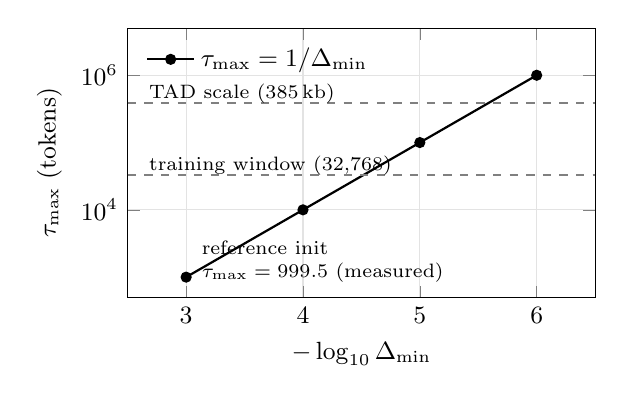
\begin{tikzpicture}
\begin{semilogyaxis}[
  width=0.62\textwidth, height=5.0cm,
  xlabel={$-\log_{10}\Delta_{\min}$}, ylabel={$\tau_{\max}$ (tokens)},
  xmin=2.5, xmax=6.5, ymin=5e2, ymax=5e6,
  xtick={3,4,5,6}, grid=major, grid style={gray!22},
  tick label style={font=\small}, label style={font=\small},
  legend style={font=\small, at={(0.02,0.97)}, anchor=north west, draw=none, fill=none}]
\addplot[thick, black, mark=*, mark size=1.6pt]
  coordinates {(3,1000)(4,10000)(5,100000)(6,1000000)};
\addlegendentry{$\tau_{\max}=1/\Delta_{\min}$}
\addplot[dashed, gray, thick, forget plot] coordinates {(2.5,32768)(6.5,32768)};
\addplot[dashed, gray, thick, forget plot] coordinates {(2.5,385000)(6.5,385000)};
\node[font=\scriptsize, anchor=west] at (axis cs:2.6,46000) {training window (32{,}768)};
\node[font=\scriptsize, anchor=west] at (axis cs:2.6,540000) {TAD scale (385\,kb)};
\node[font=\scriptsize, anchor=west, align=left] at (axis cs:3.05,1700)
  {reference init\\$\tau_{\max}=999.5$ (measured)};
\end{semilogyaxis}
\end{tikzpicture}
\caption{The ceiling of Eq.~\eqref{eq:ceiling}. Retention time cannot exceed
$1/\Delta_{\min}$ regardless of training. At the reference
$\Delta_{\min}=10^{-3}$ the bound sits two orders of magnitude below the
training window and three below domain scale.}
\label{fig:ceiling}
\end{figure}

\paragraph{The fix, and what it costs.}
Lowering $\Delta_{\min}$ to $10^{-6}$ raises the bound to $10^{6}$ tokens. This
changes three constants and \emph{no parameters}. Table~\ref{tab:f4} reports
trained models before and after.

\begin{table}[t]
\centering\small
\caption{Effect of the initialisation fix. Three seeds per row, $2{,}000$ steps,
$32{,}768$\,bp window. Parameter count is identical across rows.}
\label{tab:f4}
\begin{tabular}{lccc}
\toprule
 & median trained $\tau$ & directions reaching TAD scale & val bits/nt \\
\midrule
reference ($\Delta_{\min}=10^{-3}$) & $14.2$ & $0/32$ & $1.5210 \pm 0.0040$ \\
corrected ($\Delta_{\min}=10^{-6}$) & $\mathbf{434.7}$ & $\mathbf{32/32}$ & $1.5197 \pm 0.0025$ \\
\bottomrule
\end{tabular}
\end{table}

\paragraph{A second constant, and why the diagnostic missed it.}
Our conditioned model (\S\ref{sec:method}) adds a permeability gate $p_t$, giving
$\tau = 1/(\Delta|A| + p)$. A floor on $p$ is a ceiling on $\tau$ exactly as
$\Delta_{\min}$ is, and with the gate bias initialised at $-4$ we have
$p = 0.0182$ and hence $\tau \le 1/p \approx 55$ tokens --- \emph{below} the
uncorrected reference bound, and applying only to the conditioned arm.

This went undetected because the standard estimator computes $\tau$ from
$\Delta$ alone, omitting $p$. Under that estimator the conditioned model
reported a median $\tau$ of $487.3$ against the baseline's $434.7$, i.e.\ an
apparent \emph{lengthening}; recomputed with $p$ included, its true median is
$\approx 51$ tokens, roughly $8.5\times$ \emph{shorter}. The quantity being
reported was not the quantity governing memory.

We state this as a general caution. In any selective SSM, every additive term
entering the discretisation imposes its own reciprocal ceiling, and a $\tau$
diagnostic that omits one will report a plausible number that is not the model's
memory. We found two such constants in one architecture.

\section{Structure-conditioned pretraining}
\label{sec:method}

\begin{figure}[t]
\centering
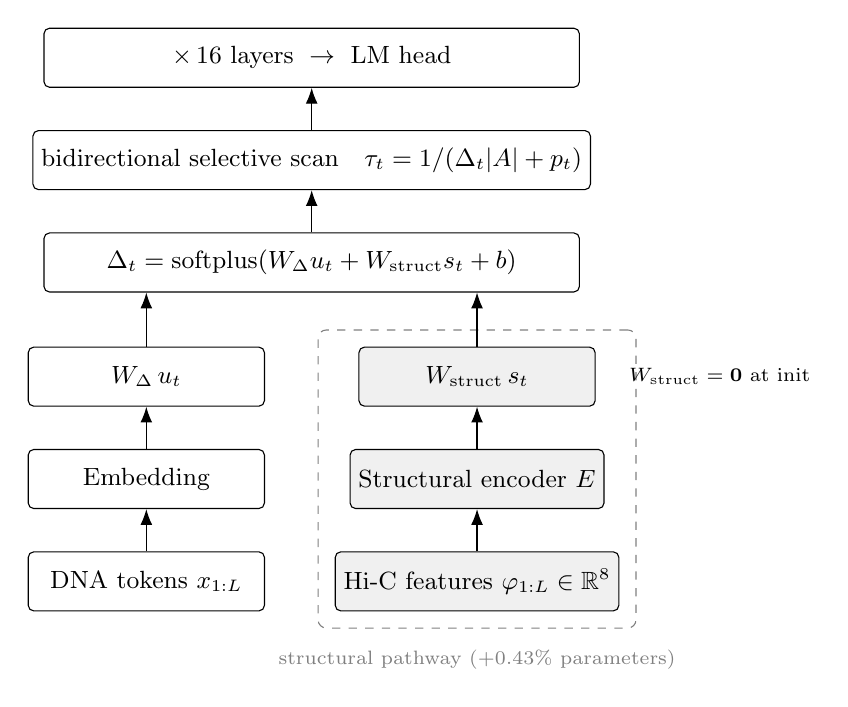
\begin{tikzpicture}[
  font=\small, node distance=0pt,
  box/.style={draw, rounded corners=2pt, minimum height=7.5mm, minimum width=30mm,
              align=center, inner sep=3pt},
  sh/.style={draw, fill=black!6, rounded corners=2pt, minimum height=7.5mm,
             minimum width=30mm, align=center, inner sep=3pt},
  wide/.style={draw, rounded corners=2pt, minimum height=7.5mm, minimum width=68mm,
               align=center, inner sep=3pt},
  ar/.style={-{Latex[length=2mm]}, thin}]

\def\lx{-2.1}   % left  column centre
\def\rx{2.1}    % right column centre

% left (sequence) column, bottom-up
\node[box]  (tok)  at (\lx, 0.0) {DNA tokens $x_{1:L}$};
\node[box]  (emb)  at (\lx, 1.3) {Embedding};
\node[box]  (proj) at (\lx, 2.6) {$W_\Delta\, u_t$};

% right (structural) column
\node[sh]   (phi)  at (\rx, 0.0) {Hi-C features $\varphi_{1:L}\in\mathbb{R}^{8}$};
\node[sh]   (enc)  at (\rx, 1.3) {Structural encoder $E$};
\node[sh]   (wds)  at (\rx, 2.6) {$W_{\text{struct}}\, s_t$};

% shared trunk
\node[wide] (delta) at (0, 4.05)
  {$\Delta_t=\mathrm{softplus}\!\left(W_\Delta u_t + W_{\text{struct}} s_t + b\right)$};
\node[wide] (scan)  at (0, 5.35)
  {bidirectional selective scan\quad $\tau_t = 1/(\Delta_t|A| + p_t)$};
\node[wide] (out)   at (0, 6.65) {$\times\,16$ layers $\;\rightarrow\;$ LM head};

\draw[ar] (tok) -- (emb);
\draw[ar] (emb) -- (proj);
\draw[ar] (phi) -- (enc);
\draw[ar] (enc) -- (wds);
\draw[ar] (proj.north) -- ($(delta.south)+(-2.1,0)$);
\draw[ar] (wds.north)  -- ($(delta.south)+(2.1,0)$);
\draw[ar] (delta) -- (scan);
\draw[ar] (scan) -- (out);

\node[font=\scriptsize, anchor=west] at ($(wds.east)+(3mm,0)$)
  {$W_{\text{struct}}=\mathbf{0}$ at init};
\begin{scope}[on background layer]
\node[fit=(phi)(enc)(wds), draw, dashed, gray, rounded corners=3pt,
      inner sep=6pt] (grp) {};
\end{scope}
\node[font=\scriptsize, gray, anchor=north] at ($(grp.south)+(0,-1.5mm)$)
  {structural pathway ($+0.43\%$ parameters)};
\end{tikzpicture}
\caption{Structure enters at the timescale. The structural pathway (dashed) maps
eight Hi-C features to a two-dimensional code and adds a learned bias to
$\Delta_t$ inside the softplus, so it modulates \emph{retention} rather than
content. Because $W_{\text{struct}}$ is zero-initialised, the model is
numerically identical to the sequence-only baseline at step $0$.}
\label{fig:arch}
\end{figure}

The backbone is a bidirectional Mamba masked language model: $d_{\text{model}}
= 256$, $16$ layers, $d_{\text{state}} = 16$, expansion $2$, one token per base
pair, trained to reconstruct masked nucleotides. The uniform-random loss floor
is exactly $2.000$ bits/nt.

Structural conditioning adds a pointwise encoder $E: \mathbb{R}^{8} \to
\mathbb{R}^{2}$ and, per layer, a matrix $W_{\text{struct}}$ whose output is
added to the pre-activation of $\Delta$ (Fig.~\ref{fig:arch}):
\begin{equation}
\Delta_t = \mathrm{softplus}\!\left(W_\Delta u_t + W_{\text{struct}} s_t + b_\Delta\right),
\qquad s_t = E(\varphi_t).
\end{equation}
Two design choices make the comparison interpretable. $W_{\text{struct}}$ is
\emph{zero-initialised}, so at step $0$ the conditioned model computes exactly
the baseline function and any divergence is learned. And the two arms are
\emph{paired}: a reference baseline is constructed under the same seed and copied
into every shape-matching tensor, giving $275/275$ bitwise-identical parameters
at initialisation, so seed variance is shared rather than confounded with arm.

Parameter counts are $7{,}725{,}312$ (baseline) and $7{,}758{,}354$
(conditioned), a $+0.43\%$ difference against a $5\%$ budget.

\section{Experimental setup}

\paragraph{Data.} Human chromosome 9, GM12878, Hi-C from a published
deeply-sequenced experiment set, mapped to GRCh38. Of $27{,}679$ bins at $5$\,kb,
$21{,}519$ ($77.7\%$) survive coverage filtering. Windows of $32{,}768$\,bp;
$5{,}422$ train, $274$ validation, $243$ test.

\paragraph{Protocol.} Three seeds per arm, $2{,}000$ steps, fp32 throughout,
matched on steps and tokens rather than wall clock. Across-seed standard
deviation of the baseline is $\sigma = 0.0025$ bits, and the effect-size floor
was fixed \emph{in advance} at $2\sigma = 0.0050$ bits.

\paragraph{Controls.} At evaluation only, on the trained conditioned model, we
substitute $\varphi$ with: \textsc{s0} zeros; \textsc{s1} a global permutation
across bins; \textsc{s2} a $10$\,Mb circular shift; \textsc{s3} features
recomputed from contacts resampled under a distance-matched null; \textsc{s4}
eight aligned one-dimensional sequence covariates. Controls draw from a fixed
seed distinct from the training seed, so every training seed sees the same
substituted structure.

\paragraph{Computational cost.}
Table~\ref{tab:cost} reports measured memory and step time, which bound what
window widths are reachable and therefore what fraction of the structural signal
is addressable at all (\S\ref{sec:why}). Conditioning costs $10$--$14\%$ in step
time, from the two extra encoder passes required by the reverse-complement
sign flip.

\begin{table}[t]
\centering\small
\caption{Measured memory and throughput, single device, fp32, batch $2$, with
gradient checkpointing. Single process without gradient synchronisation; these
are therefore a lower bound on distributed step time.}
\label{tab:cost}
\begin{tabular}{lccc}
\toprule
window (bp) & baseline s/step & conditioned s/step & peak memory (GiB) \\
\midrule
$32{,}768$  & $3.02$  & $3.43$  & $3.81$ \\
$65{,}536$  & $6.28$  & $7.17$  & $7.51$ \\
$131{,}072$ & $15.45$ & $16.98$ & $14.90$ \\
\bottomrule
\end{tabular}
\end{table}

\section{Results}
\label{sec:results}

\paragraph{Language modelling is unchanged.}
Table~\ref{tab:main} reports the primary comparison. The conditioned arm is
$0.0020$ bits \emph{worse}, i.e.\ $0.80\sigma$, well inside noise and with the
sign pointing away from the hypothesis. The exact two-sided permutation test
gives $p = 0.600$. We note explicitly that at three seeds per arm the minimum
attainable $p$ is $0.100$, so significance was unreachable by design; this is a
limitation of the pilot, not evidence of equivalence.

\begin{table}[t]
\centering\small
\caption{Primary result. Matched parameters, matched compute, paired
initialisation. Three seeds per arm.}
\label{tab:main}
\begin{tabular}{lccc}
\toprule
 & val bits/nt & median $\tau$ (reported) & per-seed \\
\midrule
baseline & $\mathbf{1.5197 \pm 0.0025}$ & $434.7$ & $1.5196$ / $1.5172$ / $1.5223$ \\
structure-conditioned & $1.5217 \pm 0.0045$ & $487.3$ & $1.5266$ / $1.5177$ / $1.5209$ \\
\midrule
difference & $+0.0020$ ($0.80\sigma$) & \multicolumn{2}{c}{permutation $p = 0.600$ (floor $0.100$)} \\
\bottomrule
\end{tabular}
\end{table}

\paragraph{The channel is connected but carries almost nothing.}
Table~\ref{tab:controls} shows the input-substitution controls. Removing or
corrupting $\varphi$ changes the output measurably --- the structural input does
reach the prediction --- but the induced divergence is $\sim\!0.05\%$ of the
divergence caused by masking itself. The ordering
$\textsc{s3}\approx\textsc{s1}\approx\textsc{s2} \gg \textsc{s4}\approx\textsc{s0}$
is what one expects if divergence simply tracks the distance of substituted
values from the true ones, \textsc{s0} being the standardised mean. It shows the
input arrives; it does not show that structure is used.

\begin{table}[t]
\centering\small
\caption{Input-substitution controls at evaluation. Masking floor
$1.321\times10^{-1}$ is context for scale, not a threshold.}
\label{tab:controls}
\begin{tabular}{lccc}
\toprule
control & $\Delta$ bits & symmetric KL & flip rate \\
\midrule
\textsc{s0} zeros            & $+0.0000$ & $2.539\times10^{-5}$ & $0.0052$ \\
\textsc{s1} permuted         & $+0.0001$ & $6.334\times10^{-5}$ & $0.0073$ \\
\textsc{s2} shifted          & $+0.0001$ & $5.528\times10^{-5}$ & $0.0068$ \\
\textsc{s3} distance-matched & $+0.0001$ & $6.827\times10^{-5}$ & $0.0075$ \\
\textsc{s4} sequence-matched & $+0.0000$ & $2.874\times10^{-5}$ & $0.0052$ \\
\bottomrule
\end{tabular}
\end{table}

\paragraph{The pathway is trained but inert.}
Gradient pressure reached the structural pathway: the Frobenius norm of
$W_{\text{struct}}$ is non-zero in $32/32$ layer-directions in every seed
(median $0.19$--$0.22$) against the exact zero it was initialised to. Yet its
contribution to the variance of $\Delta$ is negligible. Defining
$D_1 = \mathrm{Var}_t(W_{\text{struct}}s_t)/\mathrm{Var}_t(W_\Delta u_t)$ with a
pre-registered inertness threshold of $0.05$, we measure pooled medians of
$0.0004$, $0.0002$, $0.0002$ across seeds.

The permeability gate never engaged: initialised at $p = 0.018150$, its measured
mean over $2.87\times10^{8}$ evaluations was $0.017234$ / $0.017193$ /
$0.017108$, with full range $[0.0133, 0.0197]$ --- all mass in a single bin.

\paragraph{One probe does separate the arms.}
Withholding $\varphi$ at probe time and predicting within-window insulation from
hidden states after removing window identity, every conditioned seed exceeds
every baseline seed (conditioned $+0.0254$ / $+0.0303$ / $+0.0255$; baseline
$+0.0134$ / $+0.0146$ / $+0.0221$), attaining the $3$v$3$ permutation floor of
$p = 0.100$. Two caveats travel with this. Both arms sit \emph{below} a local
GC-composition floor of $+0.0802$, so this is relative rather than absolute
structural sensitivity --- a contrast between two weak predictors. And two other
targets give nothing.

\paragraph{Neither arm separates on external benchmarks.}
Internal diagnostics cannot place a model relative to the literature, so we
additionally evaluate on a standard suite of genomic classification tasks
\citep{gresova2023} under a \emph{frozen-encoder linear probe}: the pretrained
encoder is fixed, sequences are mean-pooled over positions, and a regularised
logistic regression is fitted on the resulting representations. We emphasise
that published numbers on these tasks are obtained by \emph{fine-tuning} the
whole model and are therefore not comparable to ours; a frozen probe is a lower
bound on the same weights. What the protocol does support is a floor and the
arm-versus-arm contrast, both arms receiving identical treatment.

Because these sequences have no associated Hi-C --- and two tasks are not human
--- the conditioned arm is evaluated with $\varphi$ set to zero. Its structural
pathway is therefore inactive, and any difference reflects only what
conditioning left in the sequence weights. This is the transfer setting that
matters for a foundation model: at deployment, structure is usually unavailable.

\begin{table}[t]
\centering\small
\caption{Frozen-probe accuracy on genomic classification tasks, three seeds per
arm, against a $k$-mer composition floor ($k \le 3$). Not comparable to published
fine-tuned results. Both arms exceed the composition floor; the arms do not
separate.}
\label{tab:bench}
\begin{tabular}{lccccc}
\toprule
task & $n_{\text{test}}$ & $k$-mer floor & baseline & conditioned & difference \\
\midrule
mouse enhancers & $242$ & $0.7727$ & $0.7741$ & $0.7879$ & $+0.0138$ \\
human enhancers (Cohn) & $6{,}948$ & $0.7083$ & $0.7270$ & $0.7185$ & $-0.0084$ \\
human non-TATA promoters & $9{,}034$ & $0.8083$ & $0.8413$ & $0.8418$ & $+0.0005$ \\
\bottomrule
\end{tabular}
\end{table}

Table~\ref{tab:bench} reports the completed subset. Both arms clear the
composition floor on every task, by $+0.019$ and $+0.033$ on the two with large
test sets --- evidence that pretraining on a single chromosome produced
representations exceeding trinucleotide composition. The arms do not separate:
the mean difference is $+0.0019$ accuracy, and no task exceeds $1.6$ standard
errors. We note that the largest apparent gap, on mouse enhancers, occurs on the
smallest test set, where the binomial standard error is $0.0266$ and the
observed difference is $0.52$ of it. Across eight such tasks, one arm sweeping
all three seeds of the other by chance has probability $0.57$ under the null;
we therefore do not interpret it.

\section{Why: the conditioning signal is between windows, not within them}
\label{sec:why}

The mechanism biases $\Delta$ \emph{per position}. It can therefore only exploit
variation in $\varphi$ that occurs \emph{inside} a window. We quantify the
available fraction as
\begin{equation}
\mathrm{keep}(\varphi) \;=\;
\frac{\mathbb{E}_w\left[\mathrm{Var}_{t \in w}(\varphi_t)\right]}
     {\mathrm{Var}_{t}(\varphi_t)}\,.
\end{equation}
On held-out windows $\mathrm{keep}(\varphi) = 0.0573$: $94\%$ of the structural
variance lies \emph{between} windows. The mechanism's input is nearly constant
over the interval it modulates --- by construction of the window size, not by
any failure of training.

\begin{figure}[t]
\centering
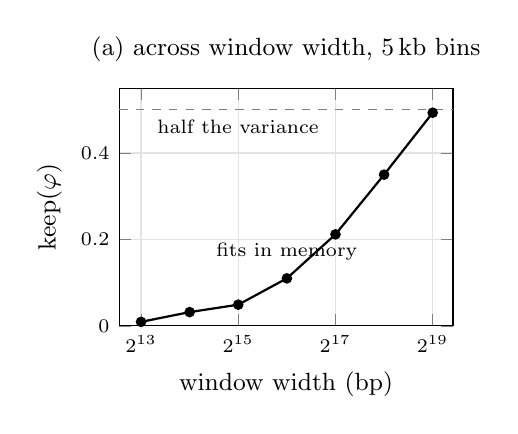
\begin{tikzpicture}
\begin{semilogxaxis}[
  width=0.48\textwidth, height=4.6cm,
  xlabel={window width (bp)}, ylabel={$\mathrm{keep}(\varphi)$},
  xmin=6000, xmax=700000, ymin=0, ymax=0.55,
  log basis x=2, grid=major, grid style={gray!22},
  tick label style={font=\scriptsize}, label style={font=\small},
  title style={font=\small}, title={(a) across window width, $5$\,kb bins}]
\addplot[thick, black, mark=*, mark size=1.5pt] coordinates {
  (8192,0.0092)(16384,0.0318)(32768,0.0490)(65536,0.1099)
  (131072,0.2117)(262144,0.3499)(524288,0.4932)};
\addplot[dashed, gray, forget plot] coordinates {(6000,0.5)(700000,0.5)};
\node[font=\scriptsize,anchor=west] at (axis cs:9000,0.46) {half the variance};
\node[font=\scriptsize,anchor=south] at (axis cs:65536,0.13) {fits in memory};
\end{semilogxaxis}
\end{tikzpicture}\hfill
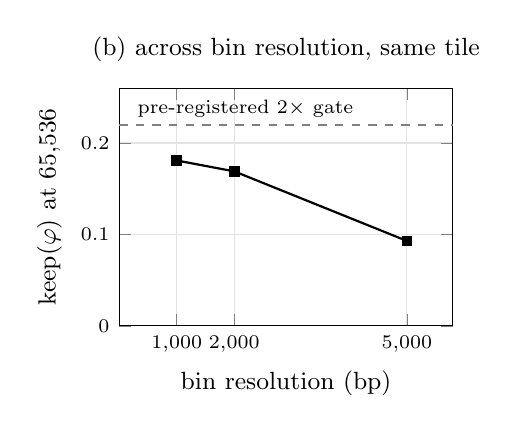
\begin{tikzpicture}
\begin{axis}[
  width=0.48\textwidth, height=4.6cm,
  xlabel={bin resolution (bp)}, ylabel={$\mathrm{keep}(\varphi)$ at $65{,}536$},
  xmin=0, xmax=5800, ymin=0, ymax=0.26,
  xtick={1000,2000,5000}, grid=major, grid style={gray!22},
  tick label style={font=\scriptsize}, label style={font=\small},
  title style={font=\small}, title={(b) across bin resolution, same tile}]
\addplot[thick, black, mark=square*, mark size=1.5pt]
  coordinates {(5000,0.0929)(2000,0.1690)(1000,0.1809)};
\addplot[dashed, gray, thick, forget plot] coordinates {(0,0.2198)(5800,0.2198)};
\node[font=\scriptsize,anchor=west] at (axis cs:150,0.238) {pre-registered $2\times$ gate};
\end{axis}
\end{tikzpicture}
\caption{The signal is between windows at every reachable setting.
(a) Widening the context raises $\mathrm{keep}(\varphi)$ but even at
$524{,}288$\,bp --- far beyond what fits in memory --- half the variance is still
between windows. (b) Refining bins five-fold on a fixed tile raises it by
$1.95\times$, missing a gate fixed in advance at $2\times$; at $1$\,kb, $81.9\%$
of the variance remains between windows.}
\label{fig:keep}
\end{figure}

Two natural remedies fail, and we measured both rather than assuming
(Fig.~\ref{fig:keep}).

\paragraph{Widening the window is a partial mitigation, not a fix.}
Across widths from $8$\,kb to $524$\,kb, $\mathrm{keep}(\varphi)$ rises
monotonically but slowly. At $65{,}536$\,bp --- which we verify fits in
$7.51$\,GiB with gradient checkpointing --- $89.0\%$ of the variance is still
between windows. At $131{,}072$\,bp, which also fits ($14.90$\,GiB) at
$2.41\times$ the step cost, $78.8\%$ remains. Even at $524{,}288$\,bp, beyond
practical memory, half of it does.

\paragraph{Refining the bins does not fix it either.}
We fetched a $10$\,Mb tile at $1$\,kb and $2$\,kb and recomputed $\varphi$ with
the same pipeline, against a same-tile $5$\,kb control. Like-for-like,
$5$\,kb $\to$ $1$\,kb raises $\mathrm{keep}(\varphi)$ at $65{,}536$\,bp by
$1.95\times$ ($0.0929 \to 0.1809$), missing a gate fixed in advance at
$2\times$. Most of the gain arrives by $2$\,kb: the final step to $1$\,kb buys
$1.071\times$ for $1.70\times$ the contact entries. At $1$\,kb bins ---
five times finer than any resolution used here --- $81.9\%$ of the variance is
\emph{still} between windows.

\paragraph{The encoder is not the bottleneck.}
One might suspect the two-dimensional structural code discards within-window
variation. It does the opposite: the ratio of $\mathrm{keep}$ after encoding to
$\mathrm{keep}$ of raw $\varphi$ is $2.21$ / $2.35$ / $1.20$ across seeds, mean
$1.92$. The encoder \emph{increases} the within-window variance fraction of what
passes through it.

\paragraph{Interpretation.}
Three independent interventions --- context length, bin resolution, and the
encoder --- leave the conclusion unchanged. The dominant variation in
Hi-C-derived features occurs on scales longer than any context these models can
process, which is a statement about the spatial autocorrelation of chromatin
contact maps rather than about one implementation. A per-position conditioning
mechanism addresses the minority share by construction. This does not show that
structure-conditioned pretraining cannot work; it shows that a per-position
coupling is the wrong instrument, and that mechanisms operating at window or
inter-window granularity are the ones with access to the remaining $80$--$90\%$.

\section{Discussion and limitations}

\paragraph{What we claim.} That SSM timescale initialisation imposes ceilings
that are invisible to the usual diagnostic, and that they are cheap to remove.
That conditioning $\Delta$ on measured structure does not improve masked
language modelling at this scale. And that the reason is measurable and
architectural rather than incidental.

\paragraph{What we do not claim.} We do not claim structure is useless for
genomic representation learning. Our conditioned arm additionally paid the
$55$-token permeability ceiling of \S\ref{sec:ceiling} that the baseline did not,
so the reported null is partly a null about a handicapped mechanism; correcting
this is the first item of ongoing work.

\paragraph{Limitations.} Three seeds per arm places the minimum attainable
permutation $p$ at $0.100$, so no significant positive was expressible.
Validation loss was still descending at $2{,}000$ steps, so this is a null from
an undertrained model. Splits are internal to one chromosome, and because Hi-C
features autocorrelate over megabases, held-out $\varphi$ leaks more than
held-out sequence --- a bias \emph{toward} the conditioned arm, which makes the
null more rather than less credible but disqualifies any positive. And the scale
is small: $7.7$M parameters, one cell line, $\approx\!0.5$B pretraining tokens.
For calibration, a comparable published bidirectional-Mamba genomic model is
parameter-matched to ours ($7.73$M, $d_{\text{model}}=256$, $16$ layers) but
pretrained on roughly $100\times$ more tokens; we compare mechanism, not scale.

\paragraph{A caution for cross-cell-line evaluation.}
Evaluating structure-aware models across cell types is the natural next test,
and a common design is to probe insulation on a held-out cell line. We advise
against it, on measured grounds. TAD boundaries are substantially conserved
across cell types, so such a probe can be passed by memorising the pretraining
cell line. The usual remedy is to probe A/B compartments instead, on the premise
that they are more cell-type-variable --- but that premise is conditional on the
pair of lines chosen. Computing all eight features on a common chromosome for
three lines, we find compartment agreement of $+0.8389$ between GM12878 and
K562 against insulation agreement of $+0.7530$: for this pair the compartment
eigenvector is \emph{more} conserved than insulation, inverting the premise.
For GM12878 against IMR90 the premise holds ($+0.6906$ versus $+0.7675$). The
distinction tracks lineage --- GM12878 and K562 are both haematopoietic, IMR90
is fibroblast.

The implication is that a cross-cell-line probe should target the
\emph{differential} between lines rather than either feature in isolation: a
model that memorised the pretraining line scores zero on a differential target
by construction. We also recommend excluding contact-density features from such
comparisons, since they show the lowest agreement across \emph{every} pair
including the two same-lineage lines --- the signature of sequencing depth and
copy-number differences rather than regulatory architecture.

\paragraph{Ongoing work.} A leakage-safe split across seven chromosomes (train
chr10--13, validate chr14--15, hold out chr9) is built and unused; five paired
seeds per arm reduce the permutation floor to $0.008$; and a window-level
conditioning arm targets the between-window share identified in
\S\ref{sec:why}. Those results are not reported here.

\section{Conclusion}

Selective state-space models carry a memory horizon fixed at initialisation, and
we found two independent constants that cap it --- one in the reference
initialisation of every Mamba-family model, one specific to an additive gate and
hidden from the standard estimator. Removing the first costs no parameters and
increases trained retention thirty-fold.

With that ceiling lifted, conditioning the timescale on measured chromatin
structure left language-modelling loss unchanged. Rather than report that as an
uninformative negative, we located its cause: the structural signal varies on
scales longer than the model's context, at every resolution and window width
reachable on current hardware, so a per-position mechanism can address only a
tenth of it. That finding constrains the design space for structure-aware
genomic models more usefully than the null alone.

\clearpage
\small
\bibliographystyle{plainnat}
\begin{thebibliography}{99}
\bibitem[Dixon et al.(2012)]{dixon2012}
J.~R. Dixon, S.~Selvaraj, F.~Yue, A.~Kim, Y.~Li, Y.~Shen, M.~Hu, J.~S. Liu, and B.~Ren.
Topological domains in mammalian genomes identified by analysis of chromatin interactions.
\emph{Nature}, 485(7398):376--380, 2012.

\bibitem[Gu and Dao(2023)]{gu2023mamba}
A.~Gu and T.~Dao.
Mamba: Linear-time sequence modeling with selective state spaces.
\emph{arXiv:2312.00752}, 2023.

\bibitem[Gresova et al.(2023)]{gresova2023}
K.~Gresova, V.~Martinek, D.~Cechak, P.~Simecek, and P.~Alexiou.
Genomic benchmarks: a collection of datasets for genomic sequence classification.
\emph{BMC Genomic Data}, 24(1):25, 2023.

\bibitem[Lieberman-Aiden et al.(2009)]{liebermanaiden2009}
E.~Lieberman-Aiden, N.~L. van Berkum, L.~Williams, et~al.
Comprehensive mapping of long-range interactions reveals folding principles of the human genome.
\emph{Science}, 326(5950):289--293, 2009.

\bibitem[Nguyen et al.(2023)]{nguyen2023hyenadna}
E.~Nguyen, M.~Poli, M.~Faizi, et~al.
HyenaDNA: Long-range genomic sequence modeling at single nucleotide resolution.
\emph{NeurIPS}, 2023.

\bibitem[Rao et al.(2014)]{rao2014}
S.~S.~P. Rao, M.~H. Huntley, N.~C. Durand, et~al.
A 3D map of the human genome at kilobase resolution reveals principles of chromatin looping.
\emph{Cell}, 159(7):1665--1680, 2014.

\bibitem[Schiff et al.(2024)]{schiff2024caduceus}
Y.~Schiff, C.-H. Kao, A.~Gokaslan, T.~Dao, A.~Gu, and V.~Kuleshov.
Caduceus: Bi-directional equivariant long-range DNA sequence modeling.
\emph{ICML}, 2024.

\bibitem[Vaswani et al.(2017)]{vaswani2017}
A.~Vaswani, N.~Shazeer, N.~Parmar, J.~Uszkoreit, L.~Jones, A.~N. Gomez,
{\L}.~Kaiser, and I.~Polosukhin.
Attention is all you need.
\emph{NeurIPS}, 2017.
\end{thebibliography}

\end{document}
